%%%%%%%%%%%%%%%%%%%%%%%%%%%%%%%%%%%%%%%%%
% "ModernCV" CV and Cover Letter
% LaTeX Template
% Version 1.11 (19/6/14)
%
% This template has been downloaded from:
% http://www.LaTeXTemplates.com
%
% Original author:
% Xavier Danaux (xdanaux@gmail.com)
%
% License:
% CC BY-NC-SA 3.0 (http://creativecommons.org/licenses/by-nc-sa/3.0/)
%
% Important note:
% This template requires the moderncv.cls and .sty files to be in the same 
% directory as this .tex file. These files provide the resume style and themes 
% used for structuring the document.
%
%%%%%%%%%%%%%%%%%%%%%%%%%%%%%%%%%%%%%%%%%

%----------------------------------------------------------------------------------------
%	PACKAGES AND OTHER DOCUMENT CONFIGURATIONS
%----------------------------------------------------------------------------------------

\documentclass[11pt,a4paper,sans]{moderncv} % Font sizes: 10, 11, or 12; paper sizes: a4paper, letterpaper, a5paper, legalpaper, executivepaper or landscape; font families: sans or roman

\usepackage[utf8]{inputenc}

\usepackage[export]{adjustbox}

\usepackage{multicol}

\moderncvstyle{casual} % CV theme - options include: 'casual' (default), 'classic', 'oldstyle' and 'banking'
\moderncvcolor{blue} % CV color - options include: 'blue' (default), 'orange', 'green', 'red', 'purple', 'grey' and 'black'

\usepackage{color}

\usepackage{hyperref}

\usepackage{lipsum} % Used for inserting dummy 'Lorem ipsum' text into the template

\usepackage[scale=0.81]{geometry} % Reduce document margins
%\setlength{\hintscolumnwidth}{3cm} % Uncomment to change the width of the dates column
%\setlength{\makecvtitlenamewidth}{10cm} % For the 'classic' style, uncomment to adjust the width of the space allocated to your name

%----------------------------------------------------------------------------------------
%	NAME AND CONTACT INFORMATION SECTION
%----------------------------------------------------------------------------------------

\firstname{Christoph} % Your first name
\familyname{Hartleb} % Your last name

% All information in this block is optional, comment out any lines you don't need
%\title{Curriculum Vitae}
%\address{Av. Granvia de l'Hospitalet, 3-5}{L'Hospitalet de Llobregat, Barcelona}
%\mobile{616 745 848}
%\phone{(000) 111 1112}
%\fax{(000) 111 1113}
%\email{quim.motger@gmail.com}
%\homepage{staff.org.edu/~jsmith}{staff.org.edu/$\sim$jsmith} % The first argument is the url for the clickable link, the second argument is the url displayed in the template - this allows special characters to be displayed such as the tilde in this example
%\extrainfo{additional information}
%\photo[70pt][0.4pt]{pictures/picture} % The first bracket is the picture height, the second is the thickness of the frame around the picture (0pt for no frame)
%\quote{}

%----------------------------------------------------------------------------------------

\begin{document}

\textit{\Huge{\textcolor{gray}{Curriculum Vitae}}}

\hrulefill
%----------------------------------------------------------------------------------------
%	PERSONAL SECTION
%----------------------------------------------------------------------------------------

\begin{multicols}{2}
  \section{Personal information}
  \cvitem{Name}{Christoph Hartleb}
  \cvitem{Place of birth}{\emph{18th May, 1989}}
  \cvitem{Address}{Gudrunstraße 119/3/15}
  \cvitem{Mobile}{+43 677 623 123 43}
  \cvitem{E-Mail}{\href{mailto:christophhartleb@gmx.at}{christophhartleb@gmx.at}}
  \cvitem{Website}{\href{https://christoph16478.github.io/my-personal-site/}{https://christoph16478.github.io/my-personal-site/}}
  \columnbreak
  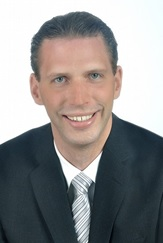
\includegraphics[width=31mm, right]{cv-picture.jpg}
\end{multicols}

%\section{Presentation}
%\cvitem{}{I'm a Computer Science Engineer with specialization in Software Engineer graduated from Facultat d'Informàtica de Barcelona (UPC). I have 3 years of experience as Java back-end software engineer, both in design/planification and implementation tasks in different international projects at the university, working alongside companies and other universities. I also have some basic experience in front-end development tools. As a freelance developer, I'm currently working in two mobile app projects, and I have some experience in web development as well.}

%----------------------------------------------------------------------------------------
%	WORK EXPERIENCE SECTION
%----------------------------------------------------------------------------------------

\section{Work experience}

%\cvlistitem{\textbf{SUPERSEDE}, \textit{Horizon 2020 Programme}. A feedback-driven approach platform for improving software's quality of service. \textbf{Tasks:} design and implementation of RESTful services; component architecture and algorithm design, implementation and extension; microservices desing and implementation; JSON formatting and data transmission using Apache Kafka; dynamic model adaptation; web front-end implementation using Spring framework.}
\cvitem{03/2020}{\textbf{Software Engineer (XML/XBRL Standards Maintainer)} \textit{Altova GmbH in Vienna,} AT}
\renewcommand{\listitemsymbol}{\textcolor{black}{-~}} % Changes the symbol used for lists
\cvlistitem{Process automation from download to preparation of XBRL taxonomies in the Taxonomy Management System: Updates on XML/XBRL taxonomies in the financial sector, download and customization of taxonomies, validation and integration of packages, finding EFM updates, adding new EDGAR rules to EDGAR support, finding schema and XML standards updates, maintaining XBRL certification}

\cvitem{2013-2014}{\textbf{Hotelbutler} \textit{Hapag Lloyd (MV Hanseatic) | Carlton Hotel in St. Moritz,} CH}
\renewcommand{\listitemsymbol}{\textcolor{black}{-~}} % Changes the symbol used for lists
\cvlistitem{Management of the suites, administration of guest databases, all-round guest care, interdepartmental cooperation}

\cvitem{2011-2013}{\textbf{Demi-Chef de Rang/Commis de Rang} \textit{Hotel Eden Roc in Ascona,} CH}
\renewcommand{\listitemsymbol}{\textcolor{black}{-~}} % Changes the symbol used for lists
\cvlistitem{Taking care of about 20 guests in one station: food service, wine service, setting the table, preparing mise en place, filleting and flambéing at the guest's table}

%\cvitem{2014--Present}{\textbf{Freelance web and mobile app developer}  Developing simple static websites for small companies and Android mobile applications.}
%\renewcommand{\listitemsymbol}{o~} % Changes the symbol used for lists
%\cvlistitem{Project: Making a commercial website using ASP.NET. Finished.}%

%\cventry{12/2013--Present}{Developer}{Bkav Corporation}{Hanoi.}{}{Developed spreadsheets for risk analysis on exotic derivatives on a wide array of commodities (ags, oils, precious and base metals), managed blotter and secondary trades on structured notes, liaised with Middle Office, Sales and Structuring for bookkeeping.
%\newline{}\newline{}
%Detailed achievements:
%\begin{itemize}
%\item Learned how to make amazing coffee
%\item Finally determined the reason for \textsc{PC LOAD LETTER}:
%\begin{itemize}
%\item Paper jam
%\item Software issues:
%\begin{itemize}
%\item Word not sending the correct data to printer
%\item Windows trying to print in letter format
%\end{itemize}
%\item Coffee spilled inside printer
%\end{itemize}
%\item Broke the office record for number of kitten pictures in cubicle
%\end{itemize}}

%----------------------------------------------------------------------------------------
%	EDUCATION SECTION
%----------------------------------------------------------------------------------------

\section{Education}

\cvitem{2017--2020}{\textbf{Master degree Digital Humanities,} \textit{University of Graz, AT}}
\cvlistitem{Key aspects: programming, web development, project management, information modelling}

\cvitem{2014--2017}{\textbf{Bachelor degree Philosophy,} \textit{University of Graz, AT}}
\cvlistitem{Key aspects: Epistemology, logic, ethics}

\cvitem{2004--2010}{\textbf{School-leaving certificate in the tourism industry,} \textit{Tourism Schools Bad Gleichenberg, AT}}
\cvlistitem{Key aspects: management}

\section{Motivation}

\cvitem{2020}{\textbf{Advanced Python Programmierung,} \textit{online learning platform Udemy}}
\cvlistitem{Functions, decorators, lambda expressions object oriented programming, exception and error handling, Cython, multiprocessing and multithreading, debugging, logging, profiling, timing and unit uesting}

\cvitem{2019}{\textbf{Der complete web developer course} \textit{online learning platform Udemy}}
\cvlistitem{HTML, CSS, JavaScript, jQuery, Twitter Bootstrap, Wordpress, PHP, MySQL, Python}

\cvitem{2019}{\textbf{Web Design for Web Developers} \textit{online learning platform Udemy}}
\cvlistitem{Design rules and principles, colors, images, fonts, visual hierarchie of objects}

%\cventry{2008--Present}{Bachelor of Computer Science}{Hanoi University of Science and Technology}{School of Information and Communication Technology, Hanoi.}{\textit{GPA -- 8.0}}{}  % Arguments not required can be left empty

%\cvitem{2011--2013}{\textbf{High School Education,} \textit{IES Baix Montseny,} Sant Celoni}

%------------------------------------------------

%\cventry{2010--2011}{Summer Intern}{\textsc{Lehman Brothers}}{Los Angeles}{}{Rated "truly distinctive" for Analytical Skills and Teamwork.}

%------------------------------------------------

%\subsection{Miscellaneous}

%\cventry{2008--2009}{Computer Repair Specialist}{Buy More}{Burbank}{}{Worked in the Nerd Herd and helped to solve computer problems by asking customers to turn their computers off and on again.}

%----------------------------------------------------------------------------------------
%	EXTRACURRICULAR SECTION
%----------------------------------------------------------------------------------------

\section{EDV - Kenntnisse}

\cvitem{}{\textbf{Programming languages:} Python, JavaScript (jQuery)}

\cvitem{}{\textbf{Markup languages:} HTML 5, XML (TEI, XPATH, DTD, RelaxNG), JSON, LaTeX}

\cvitem{}{\textbf{Stylesheet-languages:} CSS 3, Twitter Bootstrap}

\cvitem{}{\textbf{Databases and query languages:} XQuery}

\cvitem{}{\textbf{Version control:} SmartSVN, Git}

\cvitem{}{\textbf{Operating systems:} Windows 10, Ubuntu 18.10 LTS}

%\cvitem{2016}{\textbf{Training in coaching tools, }\textit{Insitut de Ciències de l'Educació}, Barcelona (10h)}
%\cvitem{Present}{\textbf{President of Hackers@UPC}, organizers of an international student hackathon hosted in UPC, Barcelona}
\

%----------------------------------------------------------------------------------------
%	SKILLS SECTION
%----------------------------------------------------------------------------------------
%\vspace{14mm}
%\section{Skills \& Background Knowledge}

%\subsection{Technical skills}

%\cvitem{}{OS admin skills in Linux and Windows}
%\cvitem{}{High skills in C, C++, Java (framework/s: Spring, Swing, Hibernate)}
%\cvitem{}{SQL and relational DBMS, and basic NoSQL knowledge}
%\cvitem{}{Web development (HTML, CSS, Javascript, PHP) and content management systems}
%\cvitem{}{Microservices and RESTful design and implementation experience}
%\cvitem{}{Amazon Web Services (web applications and database management)}
%\cvitem{}{Apache tools (Tomcat, Kafka, HTTP)}
%\cvitem{}{Android native development}
%\cvitem{}{Version control systems (Git) and build automation tools (Gradle, Maven)}
%\cvitem{}{Agile software development (use of Trello \& JIRA), testing and continuous integration}
%\cvitem{}{Advanced skills and knowledge in design patterns and software engineering}


%----------------------------------------------------------------------------------------
%	COMMUNICATION SKILLS SECTION
%----------------------------------------------------------------------------------------

%\section{Social Competence}

%\cvitem{}{High level of oral and formal written communication skills.}
%\cvitem{}{Experience and skills for team work and team leadership.}
%\cvitem{}{Outgoing and proactive.}

%----------------------------------------------------------------------------------------
%	LANGUAGES SECTION
%----------------------------------------------------------------------------------------

\section{Languages}

\cvitemwithcomment{German}{Mother tongue}{}
\cvitemwithcomment{English}{Fluent in speech and writing}{}
\cvitemwithcomment{Italian}{Very good knowledge}{}
%\cvitem{}{Institutional TOEIC: 570, Hanoi University of Science and Technology, Date taken: 18/8/2013}


%----------------------------------------------------------------------------------------
%	INTERESTS SECTION
%----------------------------------------------------------------------------------------

%\section{Interests}

%\renewcommand{\listitemsymbol}{-~} % Changes the symbol used for lists

%\cvlistitem{Cinema (member of an amateur film production company)}
%\cvlistitem{Acting (member of an amateur theatre company)}

%----------------------------------------------------------------------------------------
%	COVER LETTER
%----------------------------------------------------------------------------------------

% To remove the cover letter, comment out this entire block

%\clearpage

%\recipient{HR Department}{Corporation\\123 Pleasant Lane\\12345 City, State} % Letter recipient
%\date{\today} % Letter date
%\opening{Dear Sir or Madam,} % Opening greeting
%\closing{Sincerely yours,} % Closing phrase
%\enclosure[Attached]{curriculum vit\ae{}} % List of enclosed documents

%\makelettertitle % Print letter title

%\lipsum[1-3] % Dummy text

%\makeletterclosing % Print letter signature

%----------------------------------------------------------------------------------------

\end{document}